\subsection{GFG-8219A}


	\begin{figure}[!htb]
	\begin{minipage}{0.48\textwidth}
		\centering
		
\includegraphics[width=.7\linewidth]{../figure/GFG-8219A/main}
		
	\end{minipage}
	\hfill
	\begin{minipage}{0.48\textwidth}
		\centering
		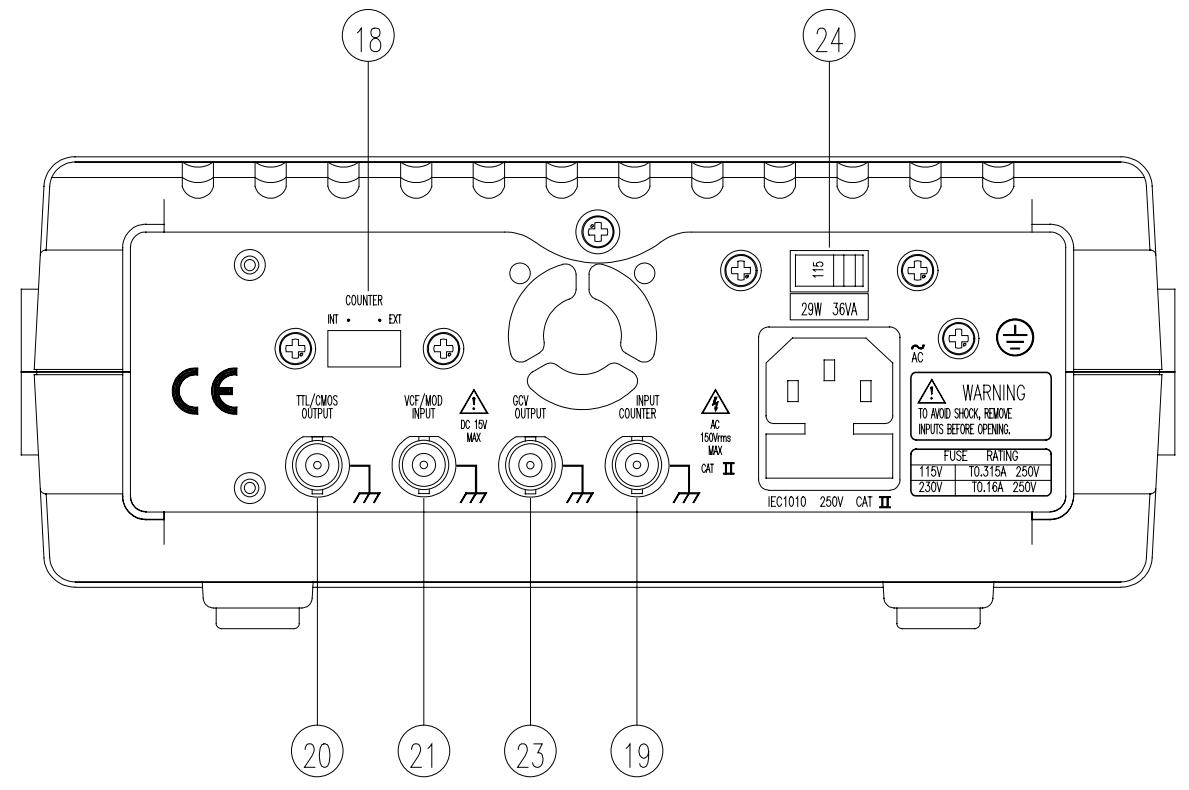
\includegraphics[width=.7\linewidth]{../figure/GFG-8219A/behind main}
		\begin{hebrew}
		\end{hebrew}
	\end{minipage}
\end{figure}

	
	\begin{enumerate}
		\item
		כפתור הפעלה
		\item
		זמן שער
		\item
		במצב מונה חיצוני, המחוון הוא
		מואר כאשר תדר המוצא גדול מ-
		הטווח שנבחר.
		\item
		מראה את התדר החיצוני
		\item
		מראה את גודל התדר באות (כמו $ K =10 ^3 $)
		\item
		מציין את זמן השער הנוכחי.
		\item
		בחירת טווח התדרים הנדרש על ידי לחיצה על
		כפתור לחיצה רלוונטי בלוח.
		\item
	לבחירת צורת הגל(מרובע,משולש,סינוסי)
		\item
		משוך החוצה וסובב את הבורר כדי להתאים את מחזור החובה של
		צורת הגל.
		\addtocounter{enumi}{1}
		\item
		משוך את הבורר כדי לבחור רמת \te{DC} כלשהי
		בין $ \pm \SI{10}{\volt}$ ,סובב עם כיוון השעון כדי להגדיר
		צורת גל ברמת \te{DC} חיובית ולהפוך לשלילה
		צורת גל ברמת \te{DC}.
		\item
		כדי לעלות או להוריד את האמפליטודה סובב עם כיוון השעון ל- \te{MAX}.
			\\
			\textbf{\te{12a}.}
		לחץ על הכפתור כדי לבצע הנחתה ב $ -\SI{20}{\decibel} $
		\item
		לחץ וסובב עם כיוון השעון את הבורר לתדר מקסימום
		והפוך לתדר מינימום.

		משוך את הכפתור כדי להתחיל את פעולת  \te{sweep}    האוטומטית
		מגבלת התדרים העליונה נקבעת על ידי הכפתור
		עמדה.
		\item
		בורר הנועד לקבוע  זמן ה\te{sweep}
		ממהיר לאיטי.
		וכדי לעבוד בצורה לוגריתמית אז יש למשוך את הבורר.
		\addtocounter{enumi}{8}
		\item
		
		זו יצאה המוציאה ערך 
		\te{DC}
		המשתנה בתלות תדר.
		
		
	\end{enumerate}

				\begin{hebrew}
		לפירוט נוסף אפשר לפנות ל:
		\href{https://datasheet.octopart.com/GDM-8245-Instek-datasheet-11997973.pdf}{\te{User Manual}}
	\end{hebrew}